\documentclass{beamer}

\usepackage[utf8x]{inputenc}
%\usepackage{default}

\usepackage{amsmath}

\usepackage{multicol}
\usepackage{url}
\usepackage{graphicx}

%figures
%\usepackage{wrapfig}

%font
\usepackage[T1]{fontenc}
\usepackage{venturis}

\usecolortheme{beaver}

%titlepage
\title{Simulation of the unstable rotation of a cuboid}
\subtitle{Books in space}
\author{Ivar Postma \and Eamon Nerbonne}
\institute[University of Groningen]
{
  Introduction to Computational Science \\
  School for Computing and Cognition \\
  University of Groningen
}
\date{January 19, 2011}

\begin{document}

\frame{\titlepage}

\begin{frame}
 \frametitle{What you should remember from last time...}
 \begin{itemize}
  \item Rotation of a rigid body; a book
  \item Clip of an experiment in space
  \item Rotation around two of the main axes is stable, rotation around the third is not
 \end{itemize}
\end{frame}

\begin{frame}
 \frametitle{String particle simulation}
 \begin{itemize}
  \item Lecture on Molecular Dynamics: simulation of vibrating string with particles
  \item Springs create interacting forces between particles
  \item From forces, calculate update velocity of points ($a = \frac{F}{m}$)
  \item From velocity, calculate update position of points
 \end{itemize}
\end{frame}

\begin{frame}
 \frametitle{Particle simulation}
 \framesubtitle{Model of a book}
 \begin{itemize}
  \item Eight particles, located at the corners
  \item Each point has the same mass
  \item Interacting force (spring) between each pair of particles
  \item Force is proportional to distance between the particles minus initial distance
 \end{itemize}
 \pause
 \begin{figure}
  \centering
  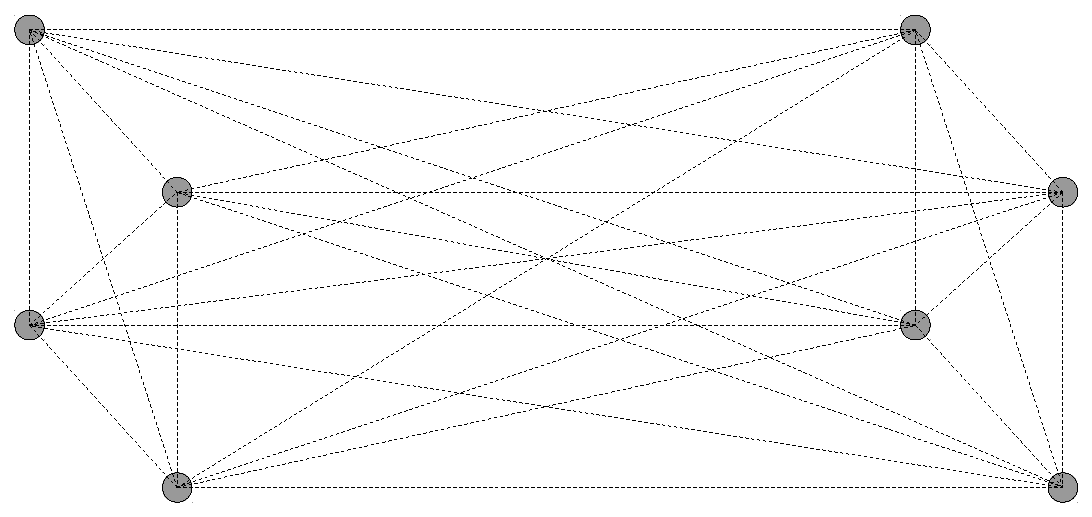
\includegraphics[width=0.7\textwidth]{strings.pdf}
 \end{figure}
\end{frame}

\begin{frame}
 \frametitle{Particle simulation}
 \framesubtitle{Computations}
 \begin{itemize}
  \item Calculate force on particle $i$:
  \begin{displaymath}
   F_i(t) = \sum_{j \neq i} k \left( \frac{\|x_i(0) - x_j(0)\|}{\|x_i(t) - x_j(t)\|} - 1\right) \left(x_i(t) - x_j(t)\right)
  \end{displaymath}
  \item Calculate velocity of particle $i$:
  \begin{displaymath}
   v_i(t + \Delta t) = v_i(t) + \frac{1}{m} F_i(t) \; \Delta t
  \end{displaymath}
  \item Calculate position of particle $i$:
  \begin{displaymath}
   x_i(t + \Delta t) = x_i(t) + v_i(t) \; \Delta t
  \end{displaymath}
 \end{itemize}
\end{frame}

\begin{frame}
 \frametitle{Particle simulation}
 \framesubtitle{Computations}
 Using Euler integration, for $n$ particles, in each time step we need to compute
 \begin{itemize}
  \item $\frac{n(n-1)}{2}$ forces
  \item $n$ velocities
  \item $n$ positions
 \end{itemize}
\end{frame}

\begin{frame}
 \frametitle{Particle simulation}
 \framesubtitle{Demonstration}
 \begin{figure}
  \centering
  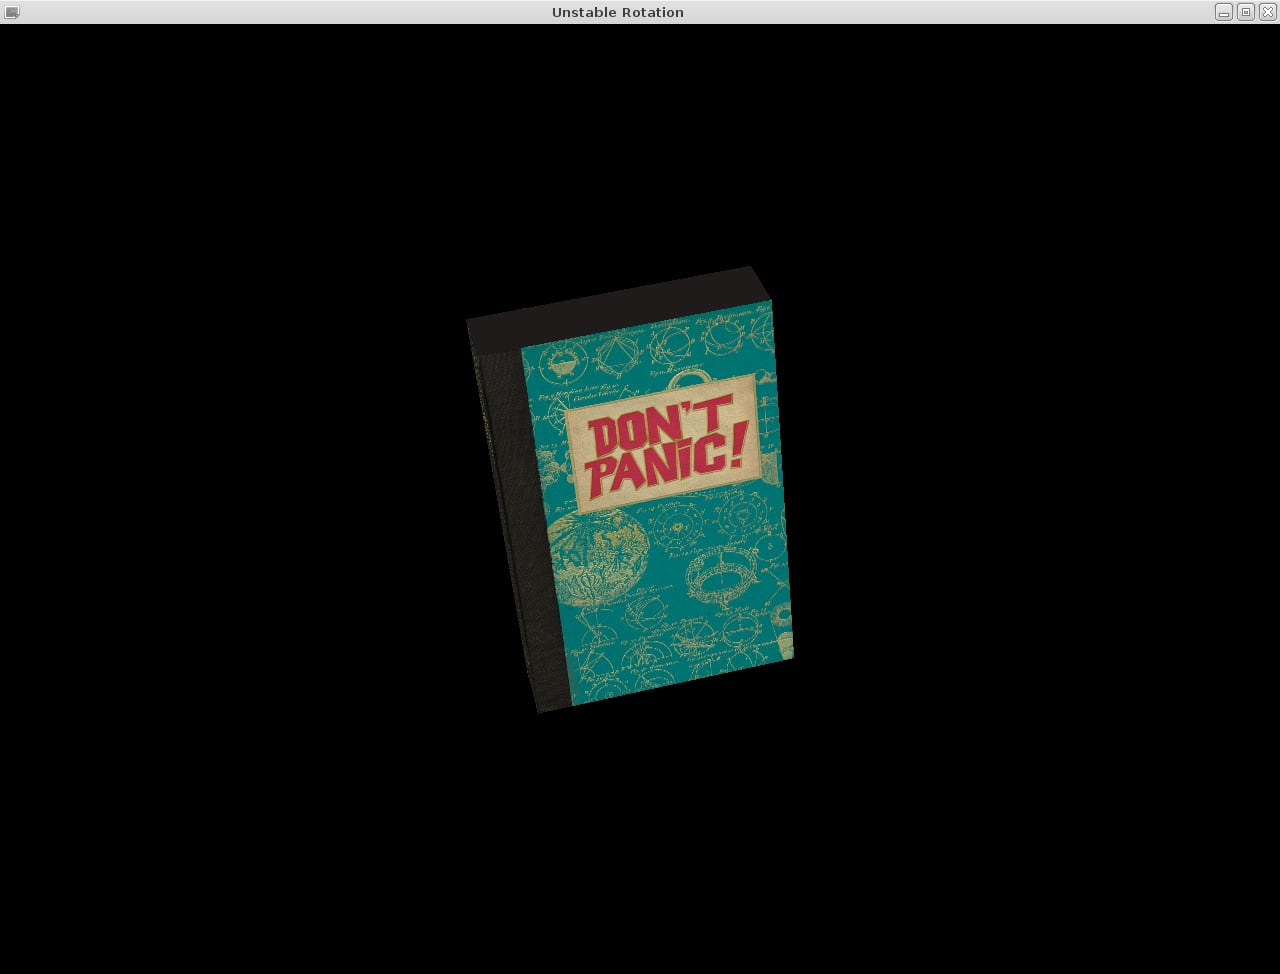
\includegraphics[width=0.7\textwidth]{demo.jpg}
 \end{figure}
\end{frame}

\begin{frame}
 \frametitle{Particle simulation}
 \framesubtitle{Observations}
 \begin{itemize}
  \item Book behaves naturally
  \item Rotation is stable around two axis and unstable around the third
  \item After some time the simulation ``explodes''
 \end{itemize}
\end{frame}

\begin{frame}
 \frametitle{Particle simulation}
 \framesubtitle{Normalisation}
 \begin{itemize}
  \item Euler integration introduces a small error in each time step
  \item Shape of book changes eventually
  \item Other techniques can reduce, but not eliminate the error
  \item Normalise the model using the conservation of energy
 \end{itemize}
\end{frame}

\begin{frame}
 \frametitle{Particle simulation}
 \framesubtitle{Demonstration with normalisation}
 \begin{figure}
  \centering
  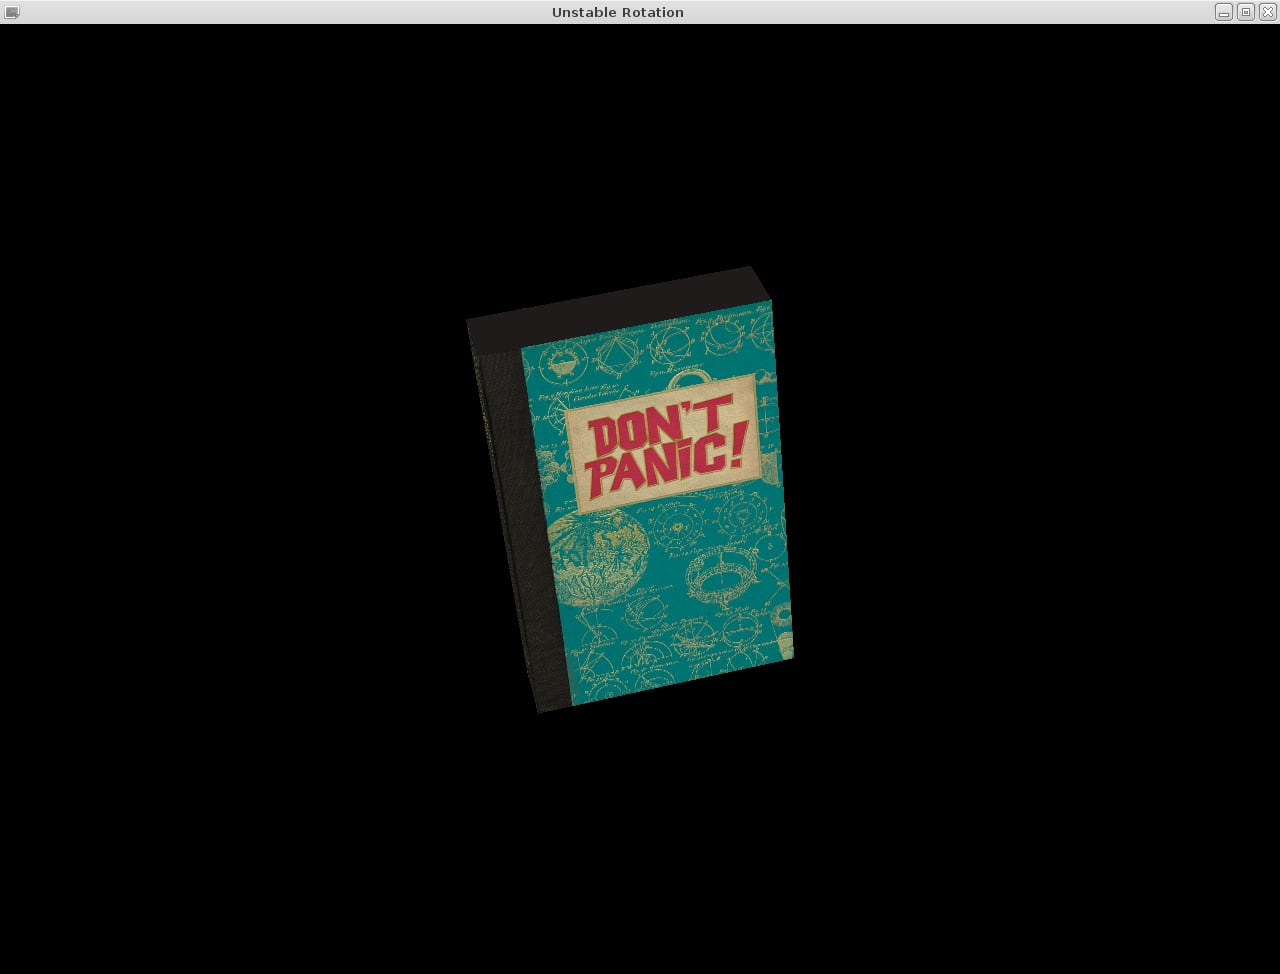
\includegraphics[width=0.7\textwidth]{demo.jpg}
 \end{figure}
\end{frame}

\begin{frame}
 \frametitle{Particle simulation}
 \framesubtitle{Normalisation}
 \begin{itemize}
  \item Energy is conserved
  \item Angular momentum is transformed into vibration
 \end{itemize}
\end{frame}

\begin{frame}
 \frametitle{A different approach}
 \begin{itemize}
  \item Different approach as introduced last time
  \item Calculate angular velocity to update the orientation
 \end{itemize}
\end{frame}

\begin{frame}
 \frametitle{Angular velocity based simulation}
 \framesubtitle{Computations}
 \begin{itemize}
  \item Angular velocity calculated from angular momentum and moment of inertia
  \begin{align*}
  I(t) &= R(t)^T \; I_{body} \; R(t) \\
  I(t)^{-1} &= R(t) \; {I_{body}}^{\!\!-1} \; R(t)^T \\
  \omega(t) &= I(t)^{-1} \; L
  \end{align*}
  \item Change in orientation calculated from angular velocity
  \begin{displaymath}
  R(t + \Delta t) = R(t) + \omega^*\!(t) \; R(t)  \;  \Delta t
  \end{displaymath}
 \end{itemize}
\end{frame}

\begin{frame}
 \frametitle{Angular velocity based simulation}
 \framesubtitle{Computations}
 Using Euler integration, in each time step we need to do
 \begin{itemize}
  \item 5 matrix multiplications
  \item 1 vector to tensor calculation
  \item 1 matrix inverse
 \end{itemize}
\end{frame}

\begin{frame}
 \frametitle{Angular velocity based simulation}
 \framesubtitle{Demonstration}
 \begin{figure}
  \centering
  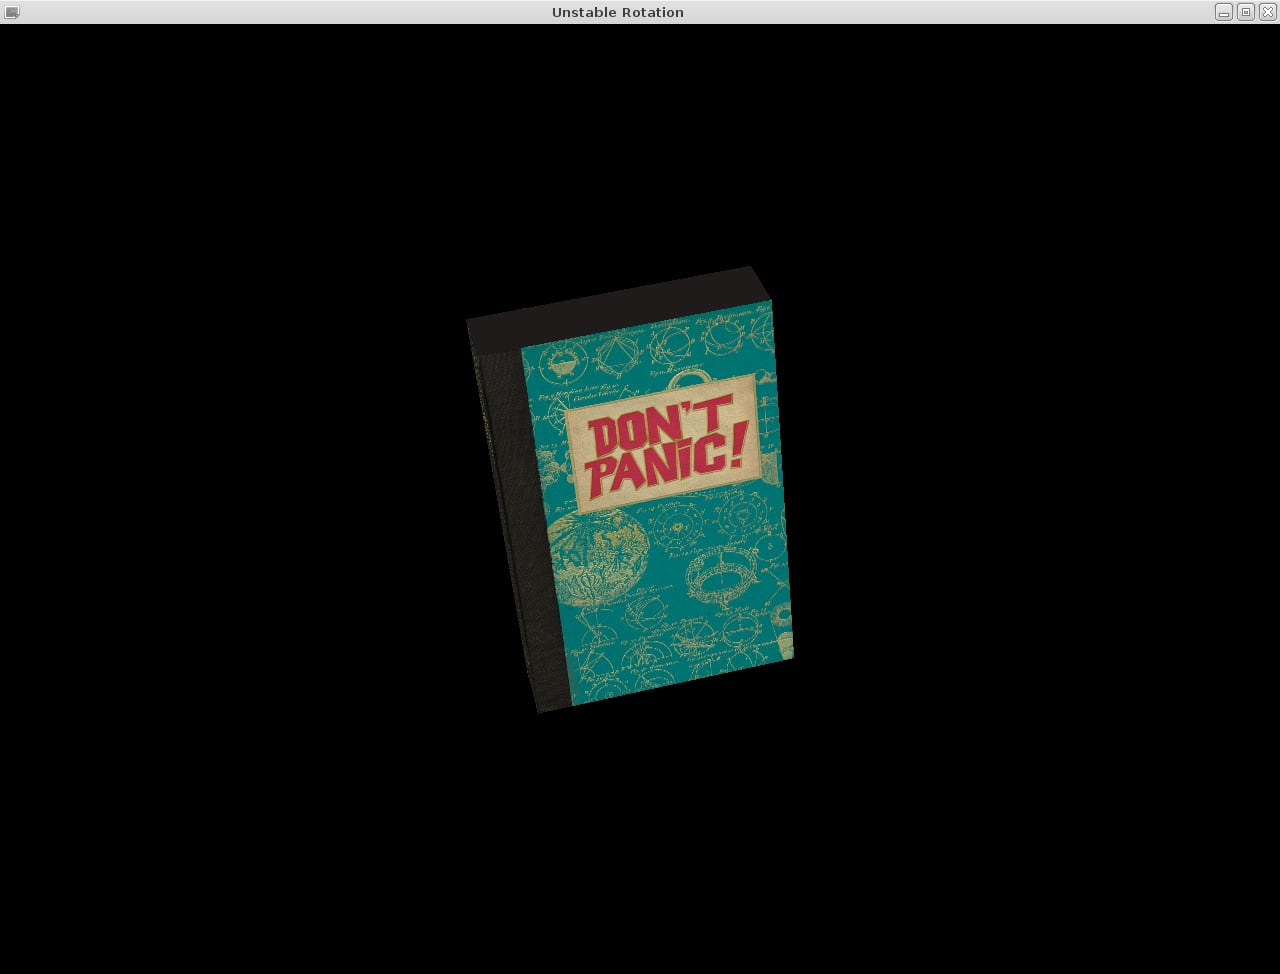
\includegraphics[width=0.7\textwidth]{demo.jpg}
 \end{figure}
\end{frame}

\begin{frame}
 \frametitle{Calculating the orientation} 
 \framesubtitle{Normalisation}
 \begin{itemize}
  \item Euler integration introduces a small error in each time step
  \item Book changes shape
  \item Orientation matrix normalised by singular value decomposition (SVD)
 \end{itemize}
\end{frame}

\begin{frame}
 \frametitle{Angular velocity based simulation}
 \framesubtitle{Demonstration with normalisation}
 \begin{figure}
  \centering
  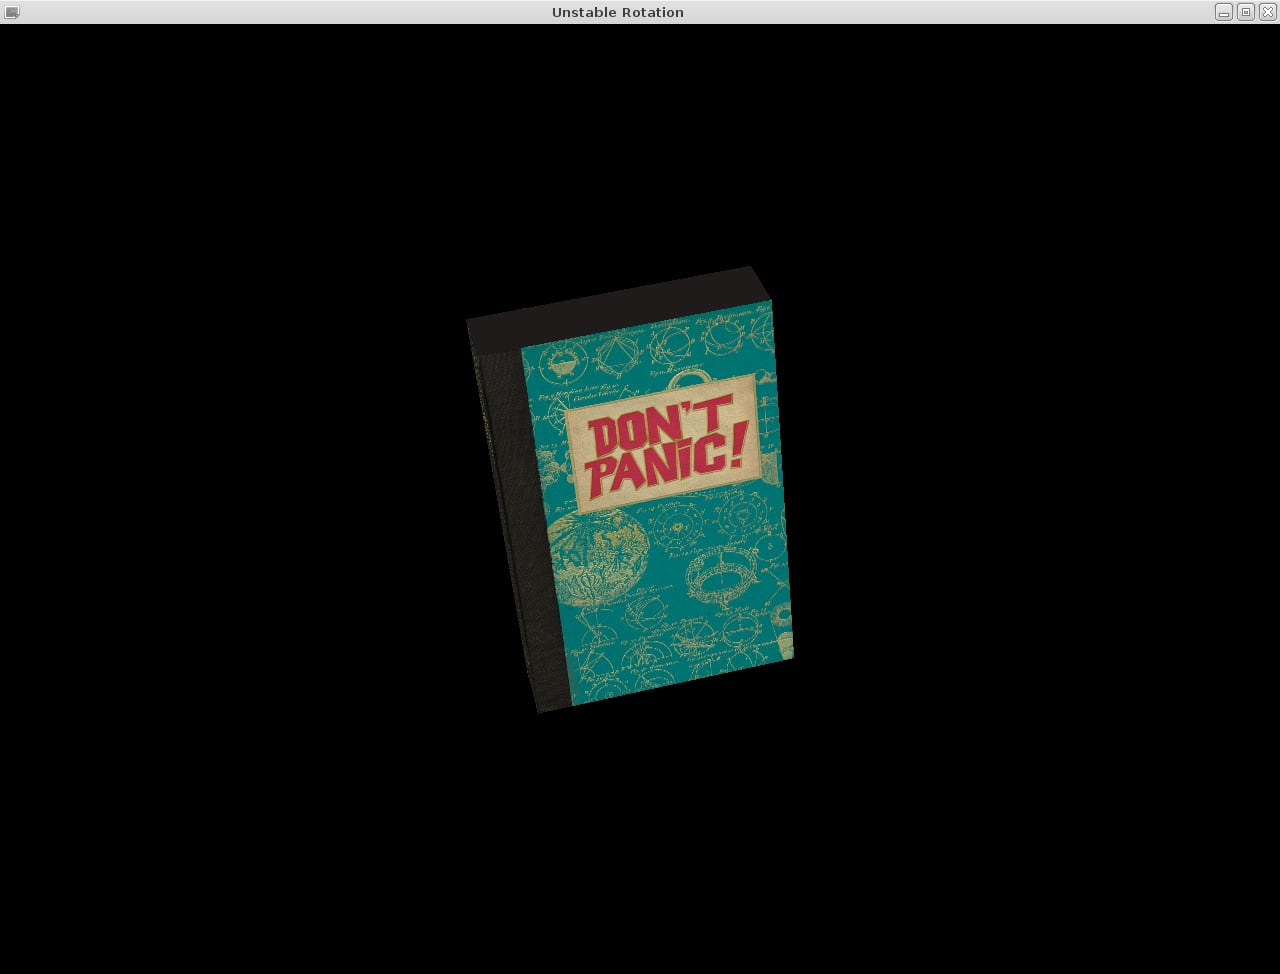
\includegraphics[width=0.7\textwidth]{demo.jpg}
 \end{figure}
\end{frame}

\begin{frame}
 \frametitle{Quaternions} 
 \begin{itemize}
  \item Orientation has 3 degrees of freedom, but a $3\times3$ matrix has 9
  \item Quaternions have 4 degrees of freedom
  \item Again, normalisation to prevent shape from changing
 \end{itemize}
\end{frame}

\begin{frame}
 \frametitle{Angular velocity based simulation}
 \framesubtitle{Demonstration with quaternions}
 \begin{figure}
  \centering
  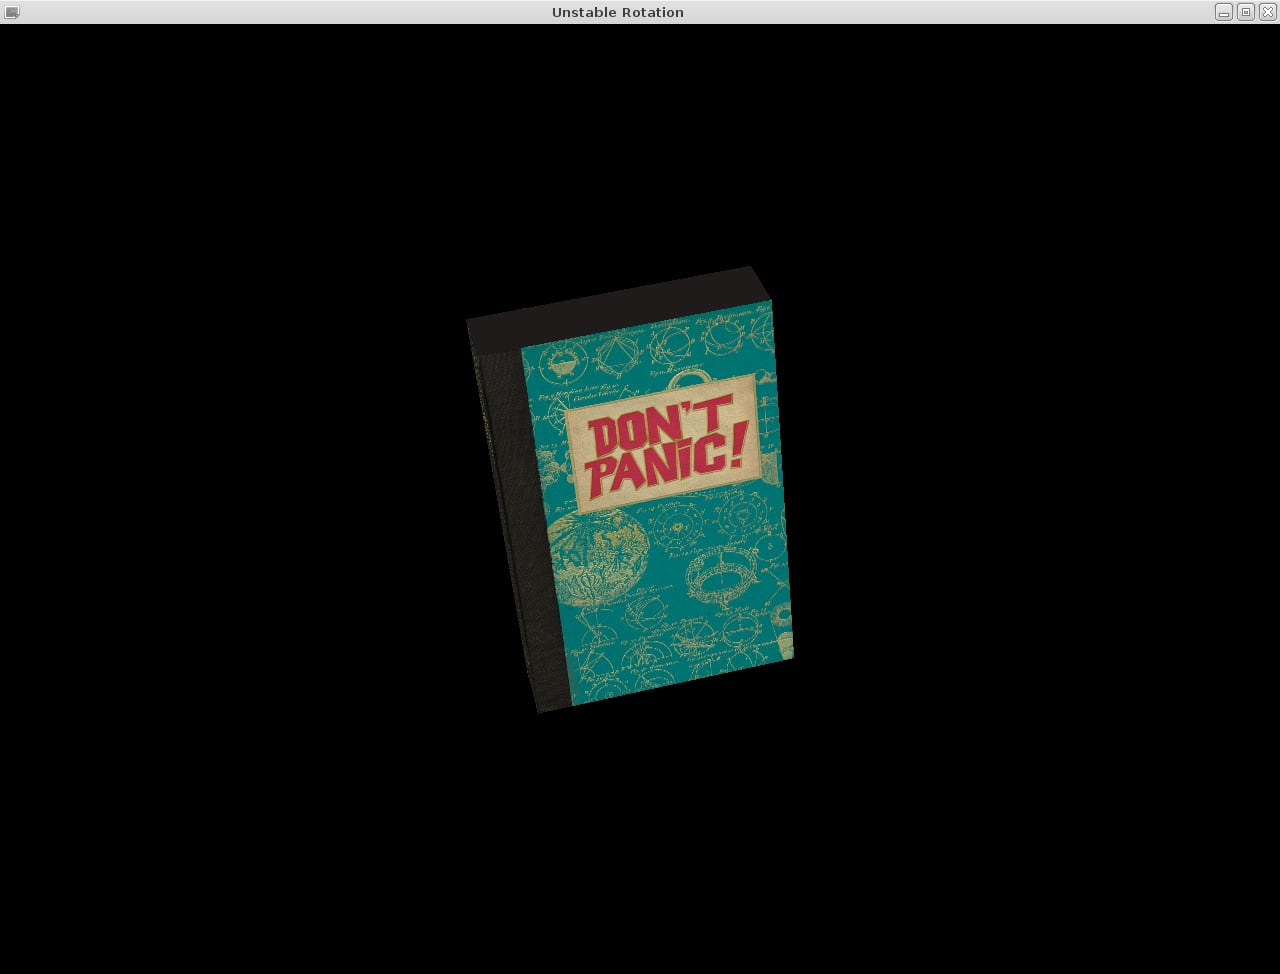
\includegraphics[width=0.7\textwidth]{demo.jpg}
 \end{figure}
\end{frame}

\begin{frame}
 \frametitle{Conclusion}
 \begin{itemize}
  \item (Un)stable rotation of a book can be simulated with particles
  \item Simulation eventually produces ``unnatural'' results
  \item Other approach preserves angular momentum
  \item Simulation is more robust
  \item Only works when moment of inertia is known
 \end{itemize}
\end{frame}

% \begin{frame}
%  \frametitle{Future work}
%  \begin{itemize}
%   \item Look at the effects of damping
%   \item Compare computational load of quaternions vs. matrix method
%  \end{itemize}
% \end{frame}

 \begin{frame}
  \frametitle{Questions?}
  \begin{center}
   \Huge{?}
  \end{center}
 \end{frame}

 \begin{frame}
  \frametitle{Questions}
  \framesubtitle{about particle simulation}
  \begin{itemize}
   \item[Q:] What happens if you change the spring constant in calculating the forces?
   \item[A:] For a high spring constant the shape and size of the book is contained better, but the book quickly goes to the vibrating state. For a low spring constant it takes longer to reach the vibrating state, but the shape and size is distorted more.
   \item[Q:] Why don't you normalise the distance between particles?
   \item[A:] If we do that, how will we calculate the forces?
  \end{itemize}
 \end{frame}

 \begin{frame}
  \frametitle{Questions}
  \framesubtitle{about particle simulation}
  \begin{itemize}
   \item[Q:] Can you improve this model?
   \item[A:] There are several extensions one can think of. For example, damping may produce better results.
  \end{itemize}
 \end{frame}

 \begin{frame}
  \frametitle{Questions}
  \framesubtitle{about quaternions}
  \begin{itemize}
   \item[Q:] What are quaternions?
   \item[A:] They're an extension to complex numbers of the form $q = a + b \cdot i + c \cdot j + d \cdot k$ that can be used to describe a rotation in 3d space. For a point at position $p(0,x,y,z)$ the position after rotation is $p'(0,x',y',z') = q \cdot p \cdot \overline{q}$.
  \end{itemize}
 \end{frame}

 \begin{frame}
  \frametitle{Questions}
  \framesubtitle{about quaternions vs. matrix method}
  \begin{itemize}
   \item[Q:] Which method is faster?
   \item[A:] In theory, quaternions produce better results and can be normalised less frequently. However, in this case the simulation is fast enough to do a normalisation in every time step.
  \end{itemize}
 \end{frame}


\end{document}
